
\begin{lemma} 
    \label{Lemma1}
    Consider three events $e$,$d$ and $k$. \\

    If
        \[
            \cons{e}{d} \ \wedge \ \reln{e}{ao}{d} \ \wedge \
            (
                (\et{d}{uo}) \ \vee \
                (\et{d}{sc} \ \wedge \ \event{d}{W})
            )
        \]        
    then,
        \[
            \reln{k}{hb}{d} \Rightarrow \reln{k}{hb}{e}.
        \]
      
    When we have two consecutive events \textit{e} and \textit{d} which are one after the other (i.e. $\reln{e}{ao}{d}$), we can use the \textit{transitive property} of $\stck{_{hb}}$ to infer that any event \textit{k} that \textit{happens before} \textit{e}, also \textit{happens before} \textit{d}. 
    However, is it possible to derive that the event \textit{k happens before e} using the evidence that \textit{k happens before d}? 
    This lemma establishes the condition when this is true.
    
\end{lemma}

%An alternative short proof 
\begin{proof}
    
    We have the following to be true:
    \begin{align*}
        cons(e,d) \ \wedge \ \reln{e}{ao}{d}.
        \tag{1}
        \label{l10}
    \end{align*}

    From \ref{l10} and by Definition of $\stck{_{hb}}$, we can infer:
    \begin{align*}
        \nexists k \ \text{s.t.} \ \reln{e}{hb}{k} \wedge \reln{k}{hb}{d}.
    \end{align*}
    from which we can conclude 
    \begin{align*}
        dir(e,d).
    \end{align*}

    Now from 
    \begin{align*}
        (\et{d}{uo}) \ \vee \
        (\et{d}{sc} \ \wedge \ \event{d}{W}).
    \end{align*}
    we can infer using Def~\ref{Dir} that for any event $k$
    \begin{align*}
        dir(k,d) \Rightarrow cons(k,d).
        \tag{2}
        \label{l11}
    \end{align*}

    Because $\stck{_{ao}}$ is a total order, $k=e$ will be the only solution satisfying \ref{l11}.  
    This means for any other $k \neq e$, we have $\neg dir(k,d)$, from which we can conclude that     
    \begin{align*}
        \reln{k}{hb}{d} \Rightarrow \reln{k}{hb}{e}.
    \end{align*}
    
    Figure~\ref{lemma:first} summarizes the intuition behind the proof.
    It showcases the direct happens-before relations that can come to $d$. 
    \begin{figure}[H]
        \centering
        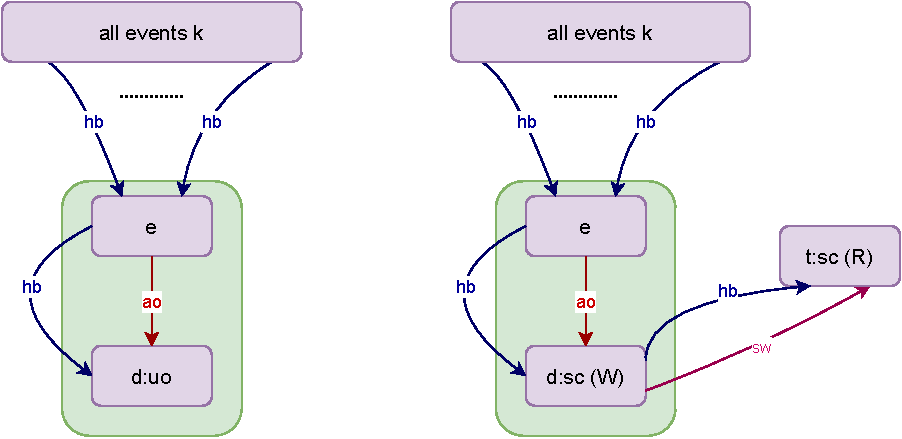
\includegraphics[scale=0.7]{4.InstructionReordering/3.Lemmas/Lemma1.pdf}
        \caption{Two cases of lemma 1 proof.}
        \label{lemma:first}
    \end{figure}
    
\end{proof}

%---------------------------------------------------------------------------------------------------------------    

%SHORTER VERSION OF PROOF WITHOUT THE ENGLISH EXPLANATION IN THE MIDDLE. DISCUSS AND DECIDE ON WHICH FORM IS BETTER
\begin{lemma}
    \label{Lemma2}
    Consider three events $e$, $d$ and $k$ \\

    If
        \[
            \cons{e}{d} \ \wedge \ \reln{e}{ao}{d} \ \wedge \
            (
                (\et{e}{uo}) \ \vee \
                (\et{e}{sc} \ \wedge \ \event{e}{R})
            )
        \]   
    then,
        \[
            \reln{e}{hb}{k} \Rightarrow \reln{d}{hb}{k}.
        \]

    When we have two consecutive events \textit{e} and \textit{d} which are one after the other (i.e. $\reln{e}{ao}{d}$), we can use the \textit{transitive property} of $\stck{_{hb}}$ to infer that any event \textit{k} that \textit{happens after} \textit{d}, also \textit{happens after} \textit{e}.
    However, is it possible to derive that the event \textit{k happens after d} using the evidence that \textit{k happens after e}? 
    This lemma states the condition when this is true.

\end{lemma}

%An alternative proof for this 
\begin{proof}
    
    We have the following to be true: 
    \begin{align*}
        cons(e,d) \ \wedge \reln{e}{ao}{d}.
        \tag{1}
        \label{l20}   
    \end{align*}

    From \ref{l20} and by Definition of $\stck{_{hb}}$, we can infer:
    \begin{align*}
        \nexists k \ \text{s.t.} \ \reln{e}{hb}{k} \wedge \reln{k}{hb}{d}.
    \end{align*}
    from which we can conclude 
    \begin{align*}
        dir(e,d).
    \end{align*}

    Now from 
    \begin{align*}
        (\et{e}{uo}) \ \vee \
        (\et{e}{sc} \ \wedge \ \event{e}{R}). 
    \end{align*}
    we can infer from Def~\ref{Dir} that for any event $k$
    \begin{align*}
        dir(e,k) \Rightarrow cons(e,k).
        \tag{2}
        \label{l21}
    \end{align*}
        
    Because $\stck{_{ao}}$ is a total order, $k=d$ will be the only solution satisfying \ref{l21}.  
    This means for any other $k \neq e$, we have $\neg dir(k,d)$, from which we can conclude that     
    \begin{align*}
        \reln{e}{hb}{k} \Rightarrow \reln{d}{hb}{k}.
    \end{align*}
     
    Figure~\ref{lemma:second} summarizes the intuition behind both cases: 
    It showcases the direct happens-before relations that can come to $e$.  
    \begin{figure}[H]
        \centering
        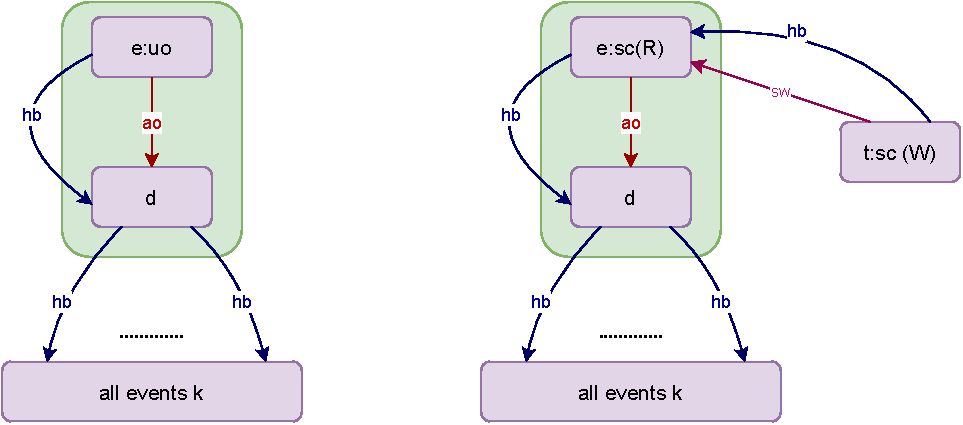
\includegraphics[scale=0.7]{4.InstructionReordering/3.Lemmas/Lemma2.pdf}
        \caption{Two cases of lemma 2 proof.}
        \label{lemma:second}
    \end{figure}

\end{proof}

%------------------------------------------------------------------------------
